\chapter{Applications}
\label{chap:applications}

In the following sections, we discuss specific lensing applications on three different scales.
Our discussion initiates with a detailed examination of microlensing events, phenomena where the gravitational field of a relatively small object, such as a star or planet, magnifies the light of a background star. This section will focus on the technique of light-curve fitting, a method that analyzes the temporal change in brightness of the lensed star to extract critical information about the lensing object. Microlensing offers a unique method for detecting elusive objects, including exoplanets \citep{sumi_unbound_2011,gaudi_microlensing_2012} and dark compact objects, providing insights into the mass, motion, and distribution of such entities within the Milky Way \citep{alcock_possible_1993,udalski_optical_1993}.

Transitioning from the stellar to the galactic scale, we next explore the realm of galaxy-scale lensing \citep{treu_strong_2010} by optimizing a parametric strong lensing model. This segment emphasizes the development and optimization of parametric models for strong lensing, where entire galaxies act as lenses, distorting and magnifying the light of more distant galaxies into arcs and rings. Through the optimization of these models, we aim to reconstruct the mass distribution of lensing galaxies \citep{auger_sloan_2010}, including the elusive dark matter component \citep{vegetti_detection_2010}. This approach not only sheds light on the structure and composition of galaxies, but also contributes to our understanding of the evolution of the large-scale structure of the Universe.

Finally, we will address weak lensing by fitting surface brightness profiles and measuring ellipticities.

% *************************************************************
%%%%% SECTION 5.1:  Fit of microlensing light curve %%%%%
\section{Microlensing light-curve fit}
\label{sec:fit_micro}

The standard microlensing light-curve, also known as the Paczynski light-curve, \citep{paczynski_gravitational_1986}, as introduced in \cref{sec:microlenses}, is defined by three parameters: the impact parameter $y_0$, the maximum magnification time $t_0$, and the Einstein radius crossing time $t_E$, which represents the time scale of the microlensing event. The latter implicitly depends on other relevant quantities of the lensing system, the lens mass $M$, the relative velocity between lens and source $v_{rel}$ and the distances between lens and source from the observer $D_L$ and $D_S$. The combination of these parameters defines the amplification to which a source with intrinsic flux $f_S$ is subjected.

The first step consists of simulating a microlensing event to obtain synthetic observational data, to which noise is then added in such a way as to mimic observational errors. We start by considering a lens with mass $M = \SI{0.3}{\msun}$ placed at a distance $D_L = \SI{4.0}{\kilo\parsec}$. We then define a source behind the lens, at a distance $D_S = \SI{8.0}{\kilo\parsec}$, characterized by an intrinsic flux of $f_S = 7.0$ (in arbitrary units), which moves with relative velocity $v_{rel} = \SI{200.0}{\kilo\meter\per\second}$ with respect to the lens. Assuming that one could monitor the source for a long period (one year in this case), a microlensing event happens when the source moves across the Einstein radius of the lens, causing a peak in the magnification. In this simulation, this occurs at $t_0 = \SI{183.0}{\day}$. After setting up the model parameters, shown in \cref{tab:parameters_micro_0}, the simulated light curve can be computed and the result is shown in \cref{fig:initial_model_micro} (black dots). The errors in the photometric measurement are assumed to be $10\%$ of the baseline flux.
Subsequently, the model was initialized with random parameters. Predictions of the model, given the set of initial parameters, are shown in \cref{fig:initial_model_micro} (red line), along with the standardized residuals, which are expressed in units of standard deviation from the mean.

\begin{figure}
  \begin{minipage}{\linewidth}
    \centering
    \subfloat[]{\includegraphics[width=\linewidth, keepaspectratio]{img/chapter5/microlensing/lc_initialmodel.png}\label{fig:lc_initialmodel}}
  \end{minipage}
  \begin{minipage}{\linewidth}
    \centering
    \subfloat[]{\includegraphics[width=\linewidth, keepaspectratio]{img/chapter5/microlensing/residuals_init.png}\label{fig:residuals_init}}
  \end{minipage}
  \caption[Microlensing initial predictions and residuals]{\protect\subref{fig:lc_initialmodel} Initial predictions of the model and \protect\subref{fig:residuals_init} residuals expressed in units of standard deviation from their mean.}
  \label{fig:initial_model_micro}
\end{figure}

\clearpage

\begin{table}[t]
\setlength{\extrarowheight}{2pt}
\setlength{\tabcolsep}{1pt}
\centering
\caption{Summary of the parameters before and after fitting the model with the set of degenerate parameters.}
\label{tab:parameters_micro_0}
%\resizebox{0.2\linewidth}{!}{
\begin{tabular}{@{}c@{\hskip 10pt}c@{}@{\hskip 10pt}c@{}@{\hskip 10pt}c@{}@{\hskip 10pt}c@{}}
\toprule
Parameter         & True value                          & Initial value                        & Best-fit value                           & Best-fit value                                                              \\
                  &                                     &                                      & (degeneracy)                             & (MCMC)                                                                      \\ \midrule
$f_S$             & \SI{7.0}{}                          & \SI{2.0}{}                           & \SI{6.993}{}                            & \SI[separate-uncertainty=true]{7.017 \pm 0.040}{}                         \\
$M$               & \SI{0.3}{\msun}                     & \SI{0.8}{\msun}                      & \SI{0.556}{\msun}                       & \SI[separate-uncertainty=true]{0.620 \pm 0.466}{\msun}                    \\
$y_0$             & \SI{0.1}{}                          & \SI{0.6}{}                           & \SI{0.100}{}                            & \SI[separate-uncertainty=true]{0.101 \pm 0.001}{}                         \\
$v_{rel}$         & \SI{200.0}{\kilo\meter\per\second}  & \SI{180.0}{\kilo\meter\per\second}   & \SI{182.881}{\kilo\meter\per\second}    & \SI[separate-uncertainty=true]{231.722 \pm 49.037}{\kilo\meter\per\second}\\
$t_0$             & \SI{183.0}{\day}                    & \SI{114.0}{\day}                     & \SI{183.002}{\day}                      & \SI[separate-uncertainty=true]{183.018 \pm 0.023}{\day}                   \\
$D_L$             & \SI{4.0}{\kilo\parsec}              & \SI{2.0}{\kilo\parsec}               & \SI{1.548}{\kilo\parsec}                & \SI[separate-uncertainty=true]{3.166 \pm 1.698}{\kilo\parsec}             \\
$D_S$             & \SI{8.0}{\kilo\parsec}              & \SI{7.0}{\kilo\parsec}               & \SI{3.786}{\kilo\parsec}                & \SI[separate-uncertainty=true]{8.658 \pm 3.457}{\kilo\parsec}             \\ \bottomrule
\end{tabular}
%}
\end{table}

After initializing the model, the cost function was defined to quantify the discrepancy between the model and the observed data. In this case, a reduced chi-square $\chi_\n^2$ was specified as the metric of choice. It is defined as
\be
\label{eq:5.01}
\chi_\nu^2 = \frac{\chi^2}{\nu} = \frac{1}{\nu} \sum\limits_{i} \bs{\frac{(O_{i} - E_{i})^2}{\s_i^2}} \,,
\ee
where $O_i$ and $E_i$ are the $i$-th observed and expected values respectively, while $\s_i$ is the data uncertainty on the $i$-th observed value. The term $\nu$ represents the degrees of freedom, calculated as the number of observations minus the number of fitted parameters. A value of $\chi_\n^2$ close to 1 suggests that the model fits the data well, with deviations between the observed and expected values largely attributable to random noise. A value significantly greater than 1 indicates that the model does not fit the data well, possibly due to systematic errors, an incorrect model, or an underestimation of the variability in the data. On the contrary, a value significantly less than 1 may suggest that the model fits the data too well, potentially due to overfitting or overestimation of the variability in the data.

At this stage, Adam \citep{kingma_adam_2017} is set as the optimizer to perform a gradient descent optimization on the cost function of choice and minimize its value by updating the model parameters at each iteration. Training starts with a loss value of $\chi_\n^2 = 192.939$ and, after 1000 iterations, the algorithm stops after reaching a $\chi_\n^2 = 1.028$.

As can be seen \cref{tab:parameters_micro_0}, even though the input parameters $f_S$, $y_0$ and $t_0$ are accurately estimated, almost matching their true values precisely, the other parameters show considerable deviation from their actual values. This discrepancy was expected and, as introduced in \cref{sec:microlenses}, is due to the high microlensing degeneracy, as these parameters collectively influence the determination of the Einstein crossing time $t_E$. In fact, it is the Einstein crossing time alone that shapes the light curve's profile.

This degeneracy can also be seen after performing a Bayesian sampling of the posterior probability distribution of the parameters using the Monte Carlo Markov Chain (MCMC) sampler implemented in the \texttt{Pyro}\footnote{\url{https://pyro.ai/}} framework \citep{bingham_pyro_2018}, which is a probabilistic programming language built on top of \texttt{PyTorch}, designed to create and run complex probabilistic models. The resulting posterior probability distributions of the parameters are shown in \cref{fig:corner_micro_bad}. In the literature, numerous methods have been known to attempt to break this degeneracy \citep{lee_microlensing_2017}. In this case, the choice was made to redefine the model so that it directly depends on $t_E$, a quantity that, as mentioned, implicitly contains all the degenerate parameters within it.

\begin{figure}
    \centering
    \includegraphics[width=\linewidth, keepaspectratio]{img//chapter5//microlensing/corner_bad.png}
    \caption[Microlensing corner plot showing degeneracy]{Corner plot showing the posterior probability distributions of the parameters used to fit the light-curve in \cref{fig:lc_initialmodel}. The projections of the probability density on planes defined by each couple of parameters, as well as one-dimensional marginalized distributions are shown. The degeneracy among the parameters $M$, $v_{rel}$, $D_L$ and $D_S$ is clearly visible.}
    \label{fig:corner_micro_bad}
\end{figure}

The fitting procedure for the simulated observations was therefore repeated, defining a model with the same initial parameters but fitting only the parameters $f_S$, $t_0$, $y_0$ and $t_E$. In this case, the initial reduced chi-square value is $\chi_\n^2 = 193.270$, and after training the model for the same number of epochs as before, it drops to a value of $\chi_\n^2 = 1.009$. The best-fit parameters are indicated in \cref{tab:parameters_micro_1}, while \cref{fig:final_model_micro,fig:micro_loss} show, respectively, the best-fit model with its standardized residuals, and the trend of the cost function as a function of the number of iterations.

\begin{table}
\setlength{\extrarowheight}{2pt}
\setlength{\tabcolsep}{1pt}
\centering
\caption{Summary of the parameters before and after fitting the model a second time to avoid degeneracy.}
\label{tab:parameters_micro_1}
%\resizebox{0.2\linewidth}{!}{
\begin{tabular}{@{}c@{\hskip 20pt}c@{}@{\hskip 20pt}c@{}@{\hskip 20pt}c@{}@{\hskip 20pt}c@{}}
\toprule
Parameter           & True value                            & Initial value                        & Best-fit value         & Best-fit value                                            \\
                    &                                       &                                      & (training)             & (MCMC)                                                    \\\midrule
$f_S$               & \SI{7.0}{}                            & \SI{2.0}{}                           & \SI{7.065}{}          & \SI[separate-uncertainty=true]{7.052 \pm 0.041}{}       \\
$M$\anote           & \SI{0.3}{\msun}                       & \SI{0.8}{\msun}                      &                        &                                                           \\
$y_0$               & \SI{0.1}{}                            & \SI{0.6}{}                           & \SI{0.103}{}          & \SI[separate-uncertainty=true]{0.100 \pm 0.001}{}       \\
$v_{rel}$\anote     & \SI{200.0}{\kilo\meter\per\second}    & \SI{180.0}{\kilo\meter\per\second}   &                        &                                                           \\
$t_0$               & \SI{183.0}{\day}                      & \SI{114.0}{\day}                     & \SI{182.989}{\day}    & \SI[separate-uncertainty=true]{183.010 \pm 0.022}{\day} \\
$D_L$\anote         & \SI{4.0}{\kilo\parsec}                & \SI{2.0}{\kilo\parsec}               &                        &                                                           \\
$D_S$\anote         & \SI{8.0}{\kilo\parsec}                & \SI{7.0}{\kilo\parsec}               &                        &                                                           \\
$t_E$               & \SI{19.1369}{\day}                    & \SI{29.3461}{\day}                   & \SI{19.025}{\day}   & \SI[separate-uncertainty=true]{19.054 \pm 0.207}{\day}  \\ \bottomrule
\end{tabular}
%}
\smallskip
\parbox[]{0.9\textwidth}{\footnotesize
  \textit{*:}
  Parameters not fitted to avoid degeneracy.
}
\end{table}

\begin{figure}
  \begin{minipage}{\linewidth}
    \centering
    \subfloat[]{\includegraphics[width=\linewidth, keepaspectratio]{img/chapter5/microlensing/best_fit.png}\label{fig:lc_finalmodel}}
  \end{minipage}
  \begin{minipage}{\linewidth}
    \centering
    \subfloat[]{\includegraphics[width=\linewidth, keepaspectratio]{img/chapter5/microlensing/residuals_best.png}\label{fig:residuals_final}}
  \end{minipage}
  \caption[Microlensing initial predictions and residuals]{\protect\subref{fig:lc_finalmodel} Predictions of the best-fit model and \protect\subref{fig:residuals_final} residuals expressed in units of standard deviation from their mean.}
  \label{fig:final_model_micro}
\end{figure}

\begin{figure}
    \centering
    \includegraphics[width=\linewidth, keepaspectratio]{img//chapter5//microlensing/corner_good.png}
    \caption[Microlensing corner plot non degenerate parameters]{As \cref{fig:corner_micro_bad} but for a model whose free parameters are $f_S$, $t_0$, $y_0$, $t_E$.}
    \label{fig:corner_micro_good}
\end{figure}

\begin{figure}[H]
    \centering
    \includegraphics[width=\linewidth, keepaspectratio]{img//chapter5//microlensing/loss.png}
    \caption[Microlensing loss value as a function of epochs]{Loss value as a function of epochs.}
    \label{fig:micro_loss}
\end{figure}

% *************************************************************
%%%%% SECTION 5.2:  Fit of microlensing light curve %%%%%
\section{Strong lens parametric reconstruction}
\label{sec:strong_lens}

This section of the thesis delves into the intricacies of parametric strong lensing, focusing on the Singular Isothermal Ellipsoid (SIE) model, a widely adopted representation for the mass distribution of lensing galaxies. The SIE model provides a robust framework for simulating gravitational lenses, offering a simplified, yet effective, portrayal of their mass profiles.

Taking advantage of the positions of multiple images generated by the lensing effect, one can derive the parameters of the lensing system that produced them. The objective is to optimize the lens parameters, which dictate the lensing behavior and, consequently, the appearance and positions of the lensed images.

This optimization is pursued through two distinct methodologies, as discussed in \cref{sec:lens_reconstruction}. Starting in both techniques from the positions of the multiple images, the first method focuses on optimizing the lens parameters within the source plane, by mapping the positions of the images back in the source plane and minimizing the distance between the theoretical and inferred position of the source.

The second method shifts the focus to the lens plane by directly minimizing the distances between each observed and predicted image to optimize the lens parameters.

\subsection{Lens modelling}
\label{subsec:lens_modelling}
The first step, as always, is to produce a simulation of the lensing system and the main observables of this topic, the multiple images of the background source.

The process begins by defining the observational parameters: a grid of $100 \times 100 \,\SI{}{\pixel}$ is established, with a resolution of $\SI{0.03}{\arcsecond\per\pixel}$. A background noise per pixel of $rms = 0.5$ mimics real observational noise. Additionally, the final image is also convolved with a Gaussian PSF with FWHM of $\SI{0.1}{\arcsecond}$. Subsequently, the definition of the lens and source hyperparameters follows. Regarding the mass distribution of the lens, an SIE model is assumed in the center of the grid, at position $(0,0)$, characterized by a velocity dispersion of $\SI{200.0}{\kilo\meter\per\second}$, axial ratio of $0.3$ and position angle of $\SI{45}{\deg}$. Concerning the surface brightness distribution, a Sérsic profile is assumed for both objects: for the lens, an effective radius of $\SI{5.0}{\arcsecond}$ and a Sérsic index $n = 3.5$, while for the source these parameters are set to $\SI{0.3}{\arcsecond}$ and $4.0$. Moreover, the source is placed at position $(-0.2 \t_E, 0.1\t_E)$ (with $\t_E$ the lens Einstein radius\footnote{$\t_E = \SI{25.92e11}{} \bp{\dfrac{\s_v^2 D_{LS}}{c^2 D_S}} \, \SI{}{\arcsecond}\,$.}), and is characterized by an axial ratio and a position angle of $0.8$ and $\SI{60}{\deg}$, respectively. We then assume that the source galaxy hosts at its center a point-like source, \eg a quasar. Finally, it is assumed that the redshifts are $z_L = 0.3$ for the lens and $z_S = 1.5$ for the source. A summary of the lens and source parameters is presented in \cref{tab:parameters_summary}.

\begin{table}[t]
\centering
\caption{Summary of lens and source parameters.}
\label{tab:parameters_summary}
\begin{minipage}{0.5\textwidth}
\vspace{0pt}
\centering
\textbf{LENS}\par\medskip
\begin{tabular}{cc}
\toprule
Parameter & Value \\
\midrule
$z_L$ & \SI{0.3}{} \\
$s_v$ & \SI{200.0}{\kilo\meter\per\second} \\
$q$ & \SI{0.3}{} \\
$\varphi$ & \SI{0.7854}{\radian} \\
$f$ & \SI{1e3}{} \\
$R_e$ & \SI{5.0}{\arcsecond} \\
$n$ & \SI{3.5}{} \\
$x_{1c}$ & \SI{0.0}{\arcsecond} \\
$x_{2c}$ & \SI{0.0}{\arcsecond} \\
\bottomrule
\end{tabular}
\label{tab:lens_parameters}
\end{minipage}%
\begin{minipage}{0.5\textwidth}
\vspace{-14pt}
\centering
\textbf{SOURCE}\par\medskip
\begin{tabular}{cc}
\toprule
Parameter & Value \\
\midrule
$z_S$ & \SI{1.5}{} \\
$q$ & \SI{0.8}{} \\
$\varphi$ & \SI{1.0472}{\radian} \\
$f$ & \SI{4.5e3}{} \\
$R_e$ & \SI{0.3}{\arcsecond} \\
$n$ & \SI{4.0}{} \\
$y_{1c}$ & \SI{-0.1676}{\arcsecond} \\
$y_{2c}$ & \SI{0.0838}{\arcsecond} \\
\bottomrule
\end{tabular}
\label{tab:source_parameters}
\end{minipage}
\end{table}

By inserting these parameters into the model, it is possible to obtain all characteristics of the lens, but the first step required to simulate the strong lensing event is to solve the lens equation for the assigned position of the source, treated at this stage as point-like. This allows the positions of the multiple images produced to be assigned to the lens plane.


\subsection{Solving the lens equation}
\label{subsec:solving_lens_eq}
Given the complexity of the model, the best solution is to solve the lens equation numerically. To do this, the method proposed by \cite{kormann_isothermal_1994} has been adopted to solve the lens equation in the case of SIE models.
Starting with the two coordinates of the source (and considering $(x, \phi)$ as the radial and angular polar coordinates.),
\begin{subequations}
\begin{align}
    \label{eq:coords1}
    y_1 & = x_1 - \a_1(\vec{x}) \,,
    \\
    \label{eq:coords2}
    y_2 & = x_2 - \a_2(\vec{x}) \,,
\end{align}
\end{subequations}
and multiplying \cref{eq:coords1} by $\cos{\phi}$ and \cref{eq:coords2} by $\sin{\phi}$ we obtain
\begin{subequations}
\begin{align}
    \label{eq:coords11}
    y_1 \cos{\phi} & = x_1 \cos{\phi} - \a_1(\vec{x}) \cos{\phi} = x \cos^2{\phi} - \a (x, \phi) \cos^2{\phi} \,,
    \\
    \label{eq:coords22}
    y_2 \sin{\phi} & = x_2 \sin{\phi} - \a_2(\vec{x}) \sin{\phi} = x \sin^2{\phi} - \a (x, \phi) \sin^2{\phi} \,.
\end{align}
\end{subequations}

Recalling that $\a (x, \phi) = \Tilde{\Psi} (\phi)$, the angular part of the lensing potential, \cref{eq:coords11,eq:coords22} can be combined to calculate the distance from the lens center as a function of $\phi$:
\be
\label{eq:coord}
x (\phi) = y_1 \cos{\phi} + y_2 \sin{\phi} + \Tilde{\Psi} (\phi) \,.
\ee

By reinserting \cref{eq:coord} into the lens equation, and setting $q^\prime = \sqrt{1 - q^2}$, we obtain
\be
\label{eq:phi_func}
F (\phi) = \bs{y_1 + \frac{\sqrt{q}}{q^\prime} \arcsinh{\bp{\frac{q^\prime}{q} \cos{\phi}}}} \sin{\phi} - \bs{y_2 + \frac{\sqrt{q}}{q^\prime} \arcsin{\bp{q^\prime \sin{\phi}}}} \cos{\phi} = 0 \,.
\ee

The task of determining the images of a source located at the coordinates $(y1, y2)$ simplifies the identification of the roots of the function $F (\phi)$. After determining $\phi$, it can be applied to \cref{eq:coord} to calculate $x$. Analytical solutions are unattainable; thus, a numerical root-finding technique is required.

The algorithm adopted to find the roots of the function $F$ shares some similarities with Brent's method \citep{brent_algorithm_1971}. In particular, it uses a numerical technique based on the bisection method, which is a type of bracketing method. This method is used to find the roots of a continuous function. The approach is iterative and relies on the intermediate-value theorem. The bisection method provides a reliable and straightforward numerical approach to find roots with a guarantee of convergence, assuming that the initial interval indeed contains a root and the function does not change sign multiple times within the interval.

Thanks to this method, it is therefore possible to solve the lens equation to derive the positions of the multiple images and produce the simulated image of the strong lensing event.

The simulated image of the lens-source system is shown in \cref{fig:data_sl}.

\begin{figure}
  \begin{minipage}{\linewidth}
    \centering
    \subfloat[]{\includegraphics[width=0.6\linewidth, keepaspectratio]{img/chapter5/strong_lens/init_data.png}\label{fig:data_sl}}
  \end{minipage}
  \begin{minipage}{\linewidth}
    \centering
    \subfloat[]{\includegraphics[width=0.6\linewidth, keepaspectratio]{img/chapter5/strong_lens/init_data_super.png}\label{fig:data_sl_super}}
  \end{minipage}
  \caption[Simulated strong lensing event]{\protect\subref{fig:data_sl} Simulated image of a strong lensing event. The pixel scale is $\SI{0.03}{\arcsecond\per\pixel}$ and the image side length is $\SI{3}{\arcsecond}$. \protect\subref{fig:data_sl_super} The same simulated image, but with the tangential critical line (solid blue line), the cut (dashed red line) and the tangential caustic (solid red line) of the lens considered shown. The yellow dashed lines identify the lens center. The orange circles represent the positions of the multiple images obtained by solving the lens equation with the method discussed in \cref{subsec:solving_lens_eq}.}
  \label{fig:obs_sl}
\end{figure}


\subsection{Lens optimization}
Initially, the model of the lens galaxy is constrained solely by the positions of the quasar's multiple images. In practical terms, these positions, as determined from astronomical observations, are subject to a degree of imprecision. To simulate positional uncertainty, a minor scatter of $\SI{0.015}{\arcsecond}$ is introduced to the actual positions of the images.

To start the fitting process, we initialize the parameters of the SIE model to some values (see \cref{tab:parameters_sl}) and start by optimizing the lens parameter in the source plane.

\begin{table}[t]
\setlength{\extrarowheight}{2pt}
\setlength{\tabcolsep}{1pt}
\centering
\caption{Summary of the parameters before and after fitting the model using both source plane or image plane optimization.}
\label{tab:parameters_sl}
%\resizebox{0.2\linewidth}{!}{
\begin{tabular}{@{}c@{\hskip 10pt}c@{}@{\hskip 10pt}c@{}@{\hskip 10pt}c@{}@{\hskip 10pt}c@{}}
\toprule
Parameter         & True value                          & Initial value                         & Best-fit value                            & Best-fit value                            \\
                  &                                     &                                       & (Source plane opt.)                       & (Image plane opt.)                        \\ \midrule
$\s_v$            & \SI{200.0}{\kilo\meter\per\second}  & \SI{220.0}{\kilo\meter\per\second}    & \SI{200.1128}{\kilo\meter\per\second}     & \SI{200.9709}{\kilo\meter\per\second}     \\ 
$q$               & \SI{0.3}{}                          & \SI{0.7}{}                            & \SI{0.2990}{}                             & \SI{0.2952}{}                             \\
$\varphi$         & \SI{0.7854}{\radian}                & \SI{1.0472}{\radian}                  & \SI{0.7855}{\radian}                      & \SI{0.7853}{\radian}                      \\ \bottomrule
\end{tabular}
%}
\end{table}


\subsubsection{Source plane optimization}
\label{subsubsec:sl_source_plane}

The first step in the optimization process involves calculating the deflection angle at the positions of the multiple images derived by solving the lens equation. This allows them to be mapped onto the source plane. Since the initial model is generally not accurate, a ``source'' will be obtained for each of the multiple images of the quasar. It is then assumed that the best estimate for the unlensed position of the quasar is the average position of these sources. The multiple sources obtained and their average position are shown in \cref{fig:sp_pred}.

\begin{figure}
    \centering
    \includegraphics[width=0.8\linewidth, keepaspectratio]{img//chapter5//strong_lens/sp_pred.png}
    \caption[Initial sources predictions source plane optimization]{The multiple images of the source are mapped back to the source plane to multiple predicted sources (green triangles). Their mean position (purple triangle) is indicated. The solid blue curves represent the caustic and the cut of the lens model, respectively. The dashed blue curves give the true caustic and cut.}
    \label{fig:sp_pred}
\end{figure}

Subsequently, it is possible to define a cost function on the source plane that needs to be minimized. This is defined as the sum of the squared differences of the distances of the individual sources predicted from their average position.
By minimizing this cost function, it is possible to optimize the model parameters so that the multiple sources converge to a single position.

This is feasible, as always, through a training loop. After defining Adam as optimizer, training is started to minimize the cost function, which decreases from a starting value of $3.1\pwr{-1}$ to a final value of $1.1\pwr{-11}$ (see \cref{fig:sp_loss}).

In \cref{tab:parameters_sl} the best-fit results are reported. Furthermore, as can be seen in \cref{fig:best_fit_sp,fig:sp_best}, in both the source plane and the lens plane, the positions of the source and multiple images overlap. Additionally, from \cref{fig:sp_bestfit,fig:sp_bestfitimage} a clear coincidence of the caustic, cut, and critical line is visible.

\begin{figure}
  \begin{minipage}{0.49\linewidth}
    \centering
    \subfloat[]{\includegraphics[width=\linewidth, keepaspectratio]{img/chapter5/strong_lens/sp_loss.png}\label{fig:sp_loss}}
  \end{minipage}
  \begin{minipage}{0.49\linewidth}
    \centering
    \subfloat[]{\includegraphics[width=\linewidth, keepaspectratio]{img/chapter5/strong_lens/best_fit_sp.png}\label{fig:best_fit_sp}}
  \end{minipage}
  \caption[Best-fit model loss history and image positions for source plane optimization]{\protect\subref{fig:sp_loss} Loss history for source plane optimization and \protect\subref{fig:data_sl_super} best-fit image positions for the source plane optimization.}
  \label{fig:loss_best_images}
\end{figure}

\begin{figure}
  \begin{minipage}{\linewidth}
    \centering
    \subfloat[]{\includegraphics[width=0.6\linewidth, keepaspectratio]{img/chapter5/strong_lens/sp_best_fit.png}\label{fig:sp_bestfit}}
  \end{minipage}
  \begin{minipage}{\linewidth}
    \centering
    \subfloat[]{\includegraphics[width=0.6\linewidth, keepaspectratio]{img/chapter5/strong_lens/sp_best_fit_imageplane.png}\label{fig:sp_bestfitimage}}
  \end{minipage}
  \caption[Best-fit model source and image plane]{Best-fit model for the source plane optimization, visualized both \protect\subref{fig:sp_bestfit} in the source plane and \protect\subref{fig:data_sl_super} in the lens plane. On the source and lens planes are indicated the caustic, cut and critical line of the best-fit model and the true ones (which overlap).}
  \label{fig:sp_best}
\end{figure}

\subsubsection{Image plane optimization}
\label{subsubsec:image_plane_opt}

Regarding the optimization on the lens plane, the first part of the process is similar: the positions of the multiple images are mapped onto the source plane and their average position is calculated. However, unlike the process discussed previously, it is now necessary to remap the average position of the sources onto the lens plane by solving the lens equation. This allows the model-predicted positions of the multiple images to be obtained. These are shown in \cref{fig:ip_pred}.

\begin{figure}
  \begin{minipage}{\linewidth}
    \centering
    \subfloat[]{\includegraphics[width=0.6\linewidth, keepaspectratio]{img/chapter5/strong_lens/ip_pred.png}\label{fig:ip_pred}}
  \end{minipage}
  \begin{minipage}{\linewidth}
    \centering
    \subfloat[]{\includegraphics[width=0.6\linewidth, keepaspectratio]{img/chapter5/strong_lens/ip_dist.png}\label{fig:ip_dist}}
\end{minipage}
\caption[Multiple images prediction for image plane optimization]{\protect\subref{fig:ip_pred} Multiple images predicted by the model and true images superimposed on the light distribution of the image plane. \protect\subref{fig:ip_dist} Illustration in the lens plane of the multiple images predicted and observed, where each closest pair has been identified. Each black stick shows the distances between each quasar image and the closest model-predicted one. The tangential critical line of the model is represented by a solid blue curve, while the true one is shown as a dashed blue curve.}
  \label{fig:ip_preds}
\end{figure}

The process then proceeds as follows: for each observed image of the quasar, the closest predicted image from the model is identified. Then, the distance between each closest pair of predicted and observed images is measured. Such distances are shown as black sticks in \cref{fig:ip_dist}.

Once the closest pairs of images have been identified and their distance calculated, all that remains is to explore the parameter space in search of the combination of $\s_v$, $q$, and $\varphi$ that minimizes this distance, in order to make every image predicted by the model converge to the real image produced by the observed system. The cost function implemented to quantify this discrepancy between images is a $\chi^2$ in the lens plane that measures the sum of the absolute distances between each pair of images, divided by the observational error on each image position, as described in \cref{subsubsec:lens_plane_source_plane_optimization}.
With these settings, the minimization procedure starts with an initial loss value $\chi^2 = 5.05\pwr{3}$ and ends with a value of $\chi^2 = 1.56\pwr{-3}$, as reported in \cref{fig:ip_loss}. The values for the best-fit parameters are reported in \cref{tab:parameters_sl}. With these parameters, the model-predicted image positions match the observed image positions very well, as can be seen in \cref{fig:best_fit_ip}.

\begin{figure}
  \begin{minipage}{0.49\linewidth}
    \centering
    \subfloat[]{\includegraphics[width=\linewidth, keepaspectratio]{img/chapter5/strong_lens/ip_loss.png}\label{fig:ip_loss}}
  \end{minipage}
  \begin{minipage}{0.49\linewidth}
    \centering
    \subfloat[]{\includegraphics[width=\linewidth, keepaspectratio]{img/chapter5/strong_lens/ip_best.png}\label{fig:best_fit_ip}}
  \end{minipage}
  \caption[Best-fit model loss history and image positions for image plane optimization]{\protect\subref{fig:ip_loss} Loss history for image plane optimization and \protect\subref{fig:best_fit_ip} best-fit image positions for the image plane optimization.}
  \label{fig:loss_best_image_plane}
\end{figure}

Once the model has been fitted to the observational data and the best-fit parameters have been derived, these can be used to obtain information about the mass distribution of the lens.

In our particular case, the best-fit velocity dispersion results in an Einstein radius
\be
\label{eq:best_er}
\t_E = \SI{25.92e11}{} \bp{\dfrac{\s_v^2 D_{LS}}{c^2 D_S}} \SI{}{\arcsecond} = \SI{0.8379}{\arcsecond} = \SI{4.06e-6}{\radian} \,,
\ee
which, knowing the redshift $z_L = 0.3$ of the lens and so its angular diameter distance $D_L = \SI{9.5e5}{\kilo\parsec}$, can be converted into physical units:
\be
\label{eq:best_er_kpc}
R_E = \t_E D_L = \SI{3.86}{\kilo\parsec} \,.
\ee

Subsequently, we can compute the critical surface density $\S_{cr}$ from \cref{eq:2.18} as
\be
\label{eq:surfcrit}
\S_{cr} = \frac{c^2}{4 \pi G} \frac{D_S}{D_L D_{LS}} = \SI{2.41e9}{\msun\per\kilo\parsec\squared} \,,
\ee
allowing us to estimate the total mass enclosed inside the Einstein radius of the lens
\be
\label{eq:mass_er}
M(<R_E) = \pi R_E^2 \S_{cr} = \SI{1.13e11}{\msun} \,.
\ee


% *************************************************************
%%%%% SECTION 5.3:  Measuring galaxy shapes and brightness distributions %%%%%
\section{Surface brightness and galaxy shapes}
\label{sec:fit_light}

This section focuses on the significance of fitting surface brightness models to simulated/observational data within the context of weak lensing.
Accurate modeling of surface brightness profiles is of utmost importance for the analysis of weak lensing effects.

Fitting surface brightness profiles is a crucial step in weak lensing studies for several reasons. First, it allows astronomers to precisely measure the shapes and orientations of galaxies, which can be subtly distorted by the gravitational lensing effect of foreground mass distributions. These distortions, although weak and difficult to detect, carry invaluable information about the mass distribution of the lensing objects, including dark matter, which is otherwise invisible. By analyzing the statistical alignment and shape changes of background galaxies, researchers can map the mass distribution of the lensing structures, offering insights into the nature of dark matter and the large-scale structure of the Universe.

Moreover, accurate fitting of surface brightness profiles helps in separating the lensing signal from intrinsic alignments and other observational effects, enhancing the reliability of weak lensing measurements. This process is fundamental in cosmology as it contributes to the precision modeling of the Universe's expansion and the distribution of matter on cosmic scales. Thus, the methodological advancements in fitting these profiles not only refine our understanding of individual galaxy structures but also bolster the broader applications of weak lensing as a tool for probing the fundamental components and dynamics of the cosmos.

By fitting observed surface brightness profiles with theoretical models, the ellipticity and orientation of galaxy images can be precisely determined, allowing for the reconstruction of the lensing field and the mapping of the mass distribution along the line of sight.


\subsection{Fit of Sérsic profile of surface brightness}
\label{subsec:sersic_fit}

The simulated galaxy is generated from a theoretical model, incorporating noise and applying a Point Spread Function (PSF), assuming that the sky background has already been subtracted from the image.

Incorporating noise into these simulations mimics the real observational conditions faced in astronomy. Sources of noise include detection equipment, atmospheric interference in ground-based observations, and intrinsic astronomical sources of variability. By integrating noise into the simulations, the fitting algorithms are tested for robustness, ensuring they can navigate the real-world data complexities.

Additionally, applying a Point Spread Function (PSF) is crucial. The PSF models the imaging system's response, capturing the effects of the telescope, detectors, and atmosphere that may blur and distort observed images. This is particularly relevant in the context of weak lensing because the PSF anisotropies can mimic lensing-induced ellipticities, biasing the shear measurements. Simulating these effects allows the fitting algorithms to consider them when analyzing objects' surface brightness.

We assume that the sky background has been subtracted from the image. This step isolates the light from the astronomical object from ambient environmental light, including atmospheric light, scattered light from nearby stars, and the Milky Way's diffuse glow. Precise background subtraction is essential for accurate surface brightness measurements.

The most common type of parametric surface brightness model is the Sérsic profile, which, as described in \cref{subsec:sersic}, is characterized by an exponential form. This is the usual profile adopted to represent the luminosity distribution of various astronomical objects, such as galaxies, by providing a flexible mathematical framework that describes a wide range of shapes from disk-like to elliptical structures.

The Sérsic profile is expressed mathematically as follows:
\be
\label{eq:5.1}
I(R) = I_e \exp \bc{- b_n \bs{\bp{\frac{R}{R_{e}}}^{\frac{1}{n}} - 1}} \,.
\ee

Assuming $q$ is the axis ratio of the elliptical distribution, the elliptical radius $R$ is thus
\be
\label{eq:5.2}
R = \sqrt{x_r^2 + (y_r / q)^2} \,,
\ee
where $x_r$ and $y_r$ the rotated coordinates obtained by aligning the reference frame $(x,y)$ of the observer to the axes of the ellipse
\begin{equation}
\begin{aligned}
    \label{eq:5.3}
    x_r & = (x - x_0) \cos{\varphi} + (y - y_0) \sin{\varphi} \,,
    \\
    y_r & = (y - y_0) \cos{\varphi} - (x-x_0) \sin{\varphi}  \,,
\end{aligned}
\end{equation}
where $x_0$ and $y_0$ represent the coordinates of the center of the ellipse and $\varphi$ the position angle.

Optimizing the Sérsic profile means fitting its seven parameters ($I_e$, $R_e$, $n$, $x_0$, $y_0$, $q$, $\varphi$) to observational data, which requires careful consideration of the effects of instrumental and observational factors, such as the Point Spread Function (PSF).

\subsubsection{Simulation of observational data}

The first step consists of simulating the observational data. It is done by constructing a $(x,y)$ grid on the sky plane with dimensions $\SI{100}{\arcsecond} \times \SI{100}{\arcsecond}$, with a pixel scale of $\SI{0.03}{\arcsecond\per\pixel}$.

The model for simulating the galaxy light profile and the parameters needed to create the mock data are then defined. The intensity at the effective radius, $I_e$, is expressed in arbitrary units, while the effective radius $R_e$ is expressed in arcseconds, together with the center coordinates. Furthermore, the axis ratio $q$ and position angle $\varphi$ of the galaxy are defined. They are linked to the ellipticity components $e_1$ and $e_2$ by the following relations
\begin{equation}
\begin{aligned}
    \label{eq:e1e2}
    e_1 & = \frac{1 - q}{1 + q} \cos{(2\varphi)} \,,
    \\
    e_2 & = \frac{1 - q}{1 + q} \sin{(2\varphi)}  \,,
\end{aligned}
\end{equation}
and their combination gives the ellipticity of the object
\be
\label{eq:ellip}
e = \sqrt{e_1^2 + e_2^2} = \frac{1-q}{1+q} \,.
\ee

The ellipticity is related to the semi-major and semi-minor axes, which is reflected in terms of shear. In particular, it can be demonstrated that the ellipticity coincides with the reduced shear $g$:
\be
\label{eq:red_shear}
e \equiv g = \frac{\g}{1 - \k} \,.
\ee

This is the concept at the basis of weak lensing: by measuring the ellipticity of the lensed images of background sources, we can infer the lenses' mass distribution. Given that ellipticity measures shear and convergence, it is then related to the second derivatives of the lensing potential.


We can then proceed with inserting the parameters inside the model. \Cref{tab:parameters_1} report a summary of the parameters to which the model is initialized.

When the parameters are added to the model, the theoretical observational data is produced and is shown in \cref{fig:0_clean}. Additionally, in \cref{fig:0_flux}, the theoretical Sérsic profile is shown: the surface brightness as a function of distance from the galaxy center, in units of $R_e$. Subsequently, to enhance the realism of the observational model, a Gaussian noise component with mean $\m = 0.0$ and standard deviation $\s = 0.05$ was added to the image. Furthermore, the resulting surface brightness was convolved with a Point Spread Function (PSF) characterized by a Full Width at Half Maximum (FWHM) of $\SI{0.1}{\arcsecond}$. The final ``noisy'' surface brightness profile is illustrated in \cref{fig:0_noisy}.

\begin{figure}
  \begin{minipage}{\linewidth}
    \centering
    \subfloat[]{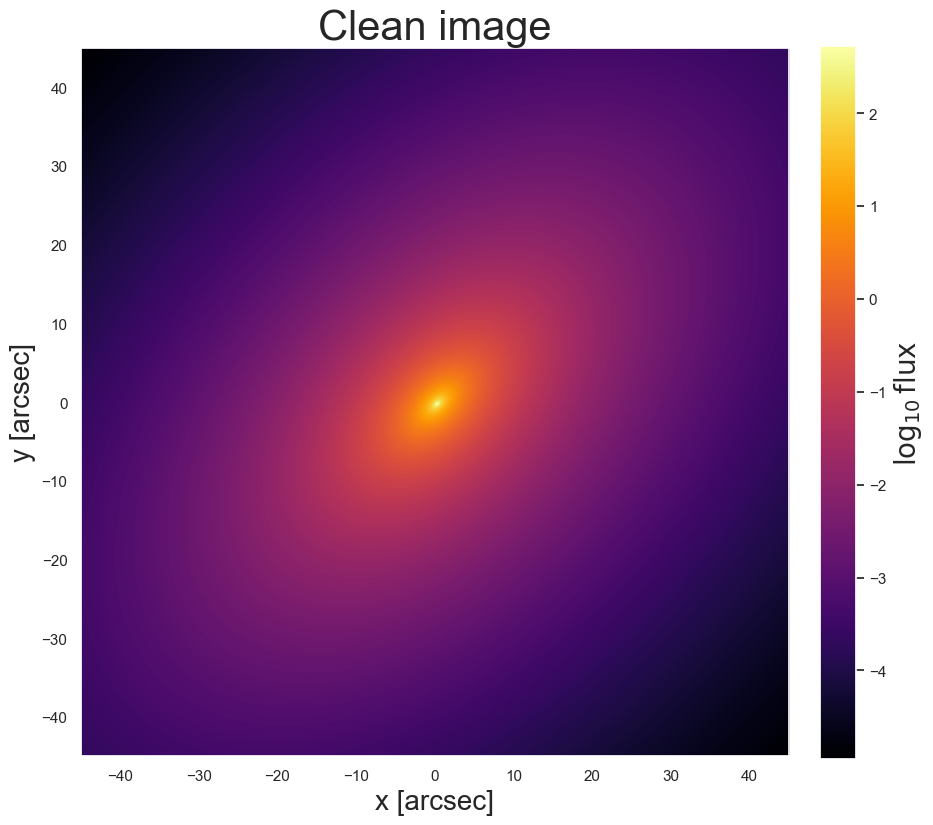
\includegraphics[width=0.75\linewidth, keepaspectratio]{img/chapter5/sersic/0_clean.png}\label{fig:0_clean}}
  \end{minipage}
  \begin{minipage}{\linewidth}
    \centering
    \subfloat[]{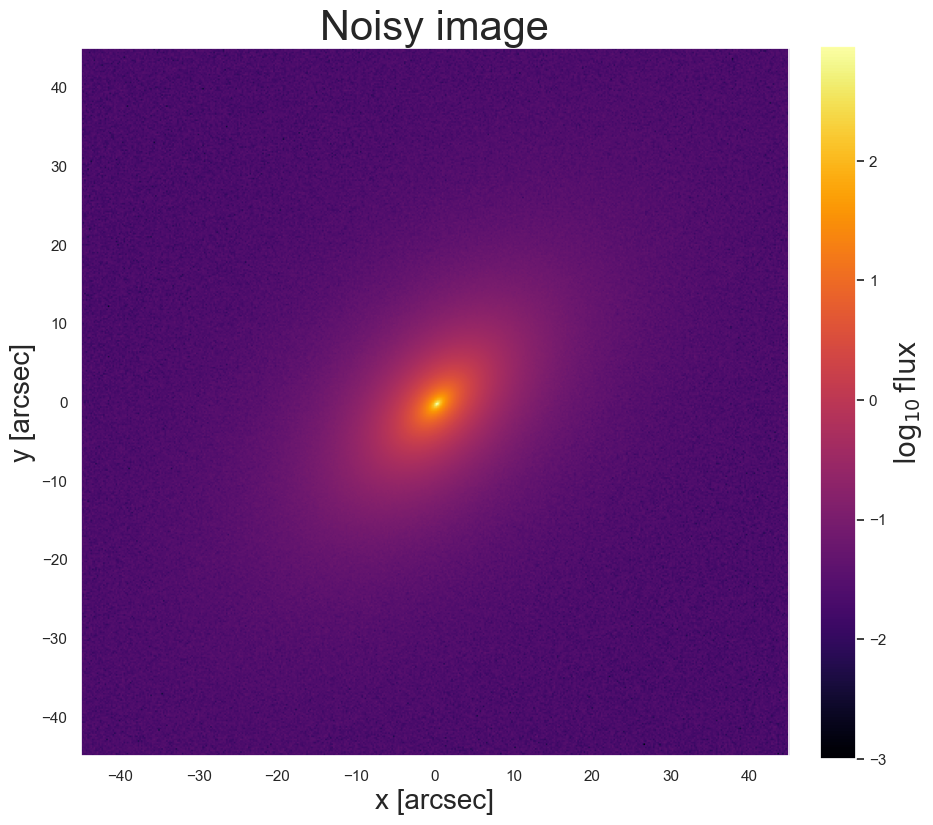
\includegraphics[width=0.75\linewidth, keepaspectratio]{img/chapter5/sersic/0_noisy.png}\label{fig:0_noisy}}
  \end{minipage}
  \caption[Simulated Sérsic surface brightness: theoretical + noisy]{Simulation of a galaxy with Sérsic surface brightness distribution: \protect\subref{fig:0_clean} theoretical model and \protect\subref{fig:0_noisy} image with Gaussian noise+PSF.}
  \label{fig:obs}
\end{figure}

\begin{figure}
    \centering
    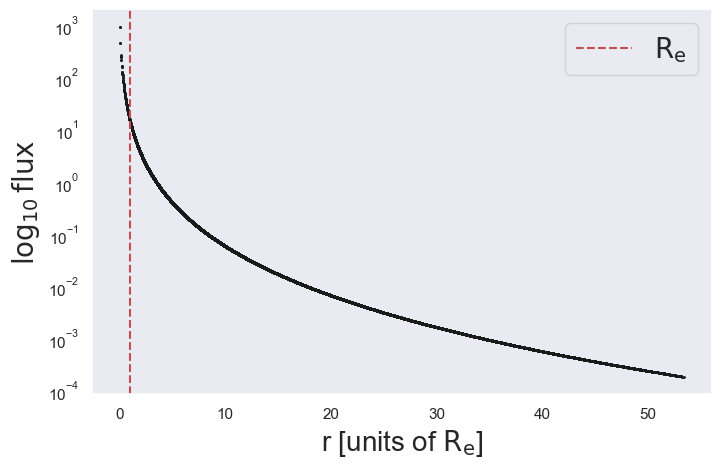
\includegraphics[width=0.8\linewidth, keepaspectratio]{img//chapter5/sersic/0_flux_r.png}
    \caption[Simulated Sérsic surface brightness vs radius]{Simulated Sérsic surface brightness distribution as a function of distance from the center of the galaxy, in units of the effective radius.}
    \label{fig:0_flux}
\end{figure}

\subsubsection{Fitting the model to data}

The next step involves fitting the model to the observational data. In this context, we establish a cost function and an optimizer, and we proceed by utilizing automatic differentiation frameworks such as PyTorch and TensorFlow. As discussed in \cref{chap:algorithms}, these components are tasked with quantifying the discrepancy between the theoretical model and the observed data and updating the model parameters by gradient descent, respectively. For this task, one of the most commonly used cost functions in regression problems, the Mean Squared Error\footnote{\url{https://pytorch.org/docs/stable/generated/torch.nn.MSELoss.html}.}\textsuperscript{,}\footnote{\url{https://www.tensorflow.org/api_docs/python/tf/keras/losses/MeanSquaredError}.} (MSE), was selected. The MSE is advantageous for its simplicity and effectiveness in quantifying the average squared discrepancy between the predicted and actual values. This makes it particularly suitable for regression tasks that aim to minimize the difference between predicted results and observed data \citep{berger_statistical_2006}.

Regarding the optimizer, Adam\footnote{\url{https://pytorch.org/docs/stable/generated/torch.optim.Adam.html}.}\textsuperscript{,}\footnote{\url{https://www.tensorflow.org/api_docs/python/tf/keras/optimizers/Adam}.} \citep{kingma_adam_2017} was chosen for its ability to combine the advantages of two other popular optimizers: AdaGrad and RMSProp \citep{tieleman_rmsprop_2014}. Adam stands out for its adaptive learning rate, which adjusts as training progresses, making it efficient for large-scale and complex problems. This adaptability is particularly beneficial for navigating complex high-dimensional data landscapes, often leading to faster convergence than other gradient descent methods.

In addition, a learning rate scheduler has been defined to improve the efficiency of model training by automatically adjusting the step $\eta$ taken by the optimizer in parameter updates\footnote{\url{https://pytorch.org/docs/stable/generated/torch.optim.lr_scheduler.ReduceLROnPlateau.html}.}\textsuperscript{,}\footnote{\url{https://www.tensorflow.org/api_docs/python/tf/keras/callbacks/ReduceLROnPlateau}.}. The initial learning rate for the optimizer is set to $\eta = 0.1$ and gradually decreases to improve the speed of finding the minimum loss function.

At this point, the model must be initialized with some initial (random) parameters that are appropriately constrained, shown in \cref{tab:parameters_1}.

\begin{table}[]
\setlength{\extrarowheight}{2pt}
\setlength{\tabcolsep}{1pt}
\centering
\caption{Summary of true and initial parameters before fitting.}
\label{tab:parameters_1}
%\resizebox{0.2\linewidth}{!}{
\begin{tabular}{@{}c@{\hskip 20pt}c@{}@{\hskip 20pt}c@{}}
\toprule
Parameter           & True value                 &  Initial value            \\ \midrule
$I_e$               & \SI{15.0}{}                &  \SI{25.0}{}              \\
$R_e$               & \SI{2.0}{\arcsecond}       &  \SI{4.5}{\arcsecond}     \\
$n$                 & \SI{5.5}{}                 &  \SI{7.0}{}               \\
$x_0$               & \SI{0.2}{\arcsecond}       &  \SI{12.2}{\arcsecond}     \\
$y_0$               & \SI{-0.3}{\arcsecond}      &  \SI{-18.0}{\arcsecond}    \\
$q$                 & \SI{0.6}{}                 &  \SI{0.8}{}               \\
$\varphi$           & \SI{0.7853}{\radian}       &  \SI{1.5708}{\radian}     \\ \bottomrule
\end{tabular}
%}
\end{table}

\begin{figure}[]
  \begin{minipage}{0.49\linewidth}
    \centering
    \subfloat[]{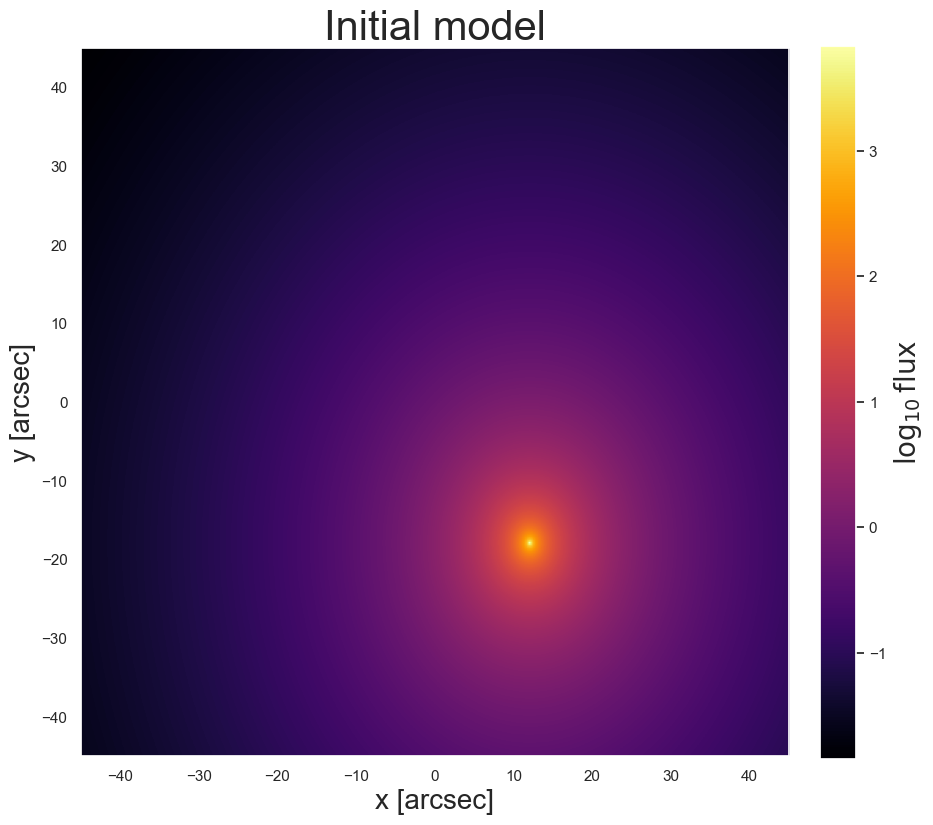
\includegraphics[width=\linewidth, keepaspectratio]{img/chapter5/sersic/1_initial.png}\label{fig:1_model_sersic}}
  \end{minipage}
  \begin{minipage}{0.49\linewidth}
    \centering
    \subfloat[]{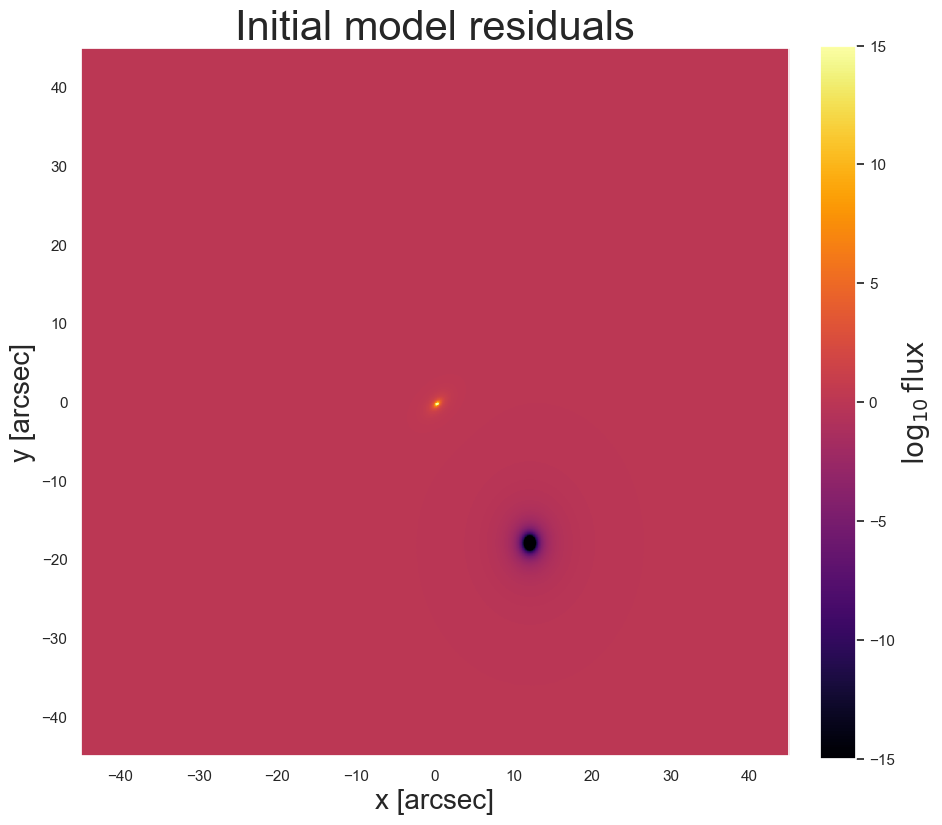
\includegraphics[width=\linewidth, keepaspectratio]{img/chapter5/sersic/1_residuals.png}\label{fig:1_model_residuals_init}}
  \end{minipage}
  \caption[Initial prediction Sérsic profile + residuals]{\protect\subref{fig:1_model_sersic} Initial prediction of Sérsic surface brightness model, computed using the initial values of \cref{tab:parameters_1} and \protect\subref{fig:1_model_residuals_init} residuals, normalized by their standard deviation, calculated as subtraction between true data and initial prediction.}
  \label{fig:1_initial}
\end{figure}

\begin{figure}
  \begin{minipage}{0.49\linewidth}
    \centering
    \subfloat[]{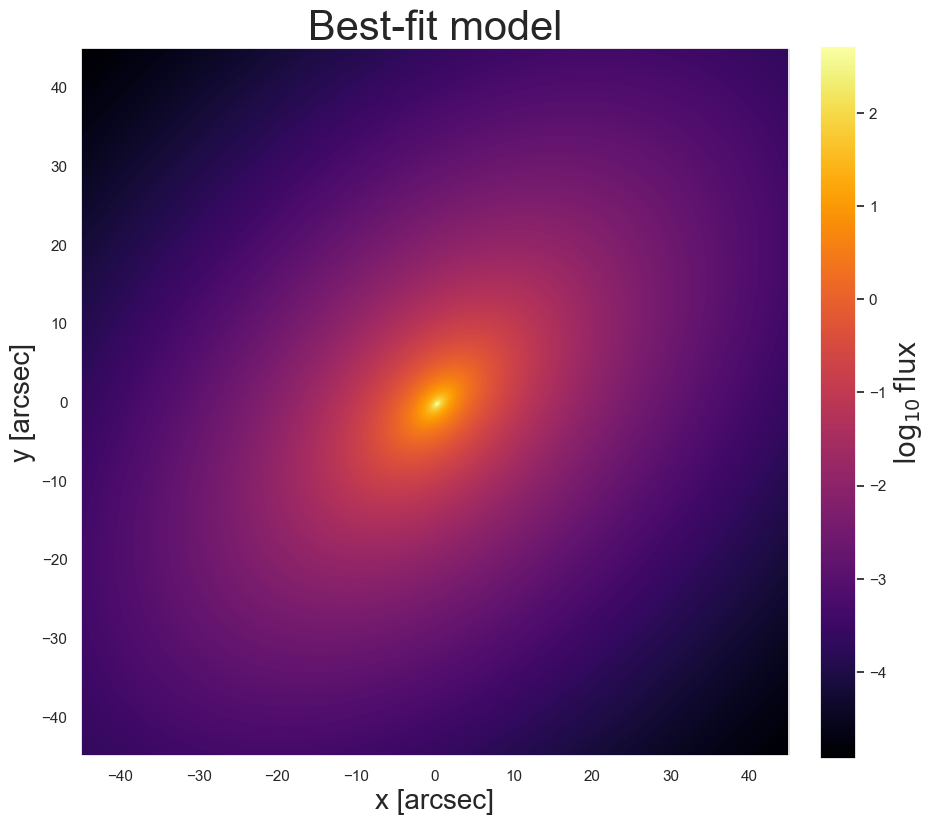
\includegraphics[width=\linewidth, keepaspectratio]{img/chapter5/sersic/sersic_best_fit.png}\label{fig:bestfit_sersic}}
  \end{minipage}
  \begin{minipage}{0.49\linewidth}
    \centering
    \subfloat[]{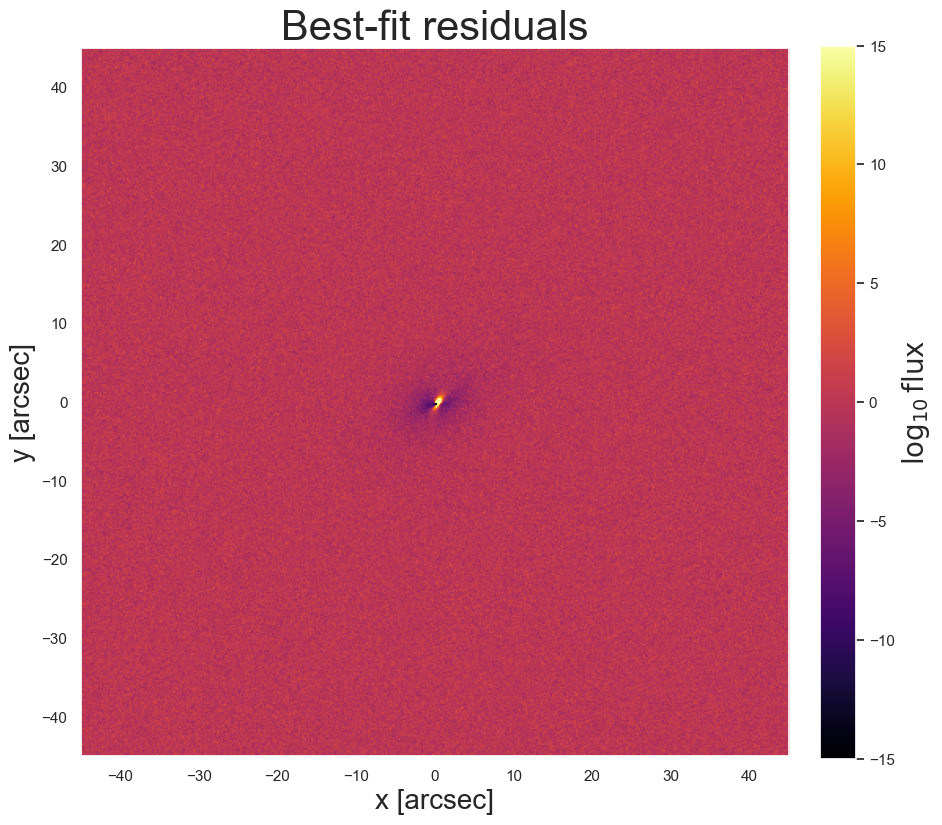
\includegraphics[width=\linewidth, keepaspectratio]{img/chapter5/sersic/res_bestfit.png}\label{fig:res_bestfit}}
  \end{minipage}
  \caption[Best-fit prediction Sérsic profile + residuals]{\protect\subref{fig:bestfit_sersic} Best-fit prediction of Sérsic surface brightness model, computed using the best-fit values of \cref{tab:parameters_2} obtained from the training process and \protect\subref{fig:res_bestfit} residuals normalized by their standard deviation, calculated as subtraction between true data and best-fit prediction.}
  \label{fig:sersic_best}
\end{figure}

The initial prediction of the model, accompanied by residuals for the actual data, is presented in \cref{fig:1_initial}. Subsequently, the model training can start. To speed up the fitting process, it is possible to minimize the cost function computed on the logarithms of the model and data as a way to normalize the data between a smaller range of values \citep{huang_normalization_2020}.

Before training the cost function, \ie the MSE between the data and the model has a value of $\mathrm{loss_{initial}} = 5.4$ and, after $50000$ iterations (or epochs) of the training loop, it drops to $\mathrm{loss_{final}} = 3.1\pwr{-10}$, reaching its absolute minimum. The best-fit parameters are reported in \cref{tab:parameters_2} and \cref{fig:loss_sersic} shows the trend of the MSE as a function of iterations of gradient descent.

\begin{figure}[]
    \centering
    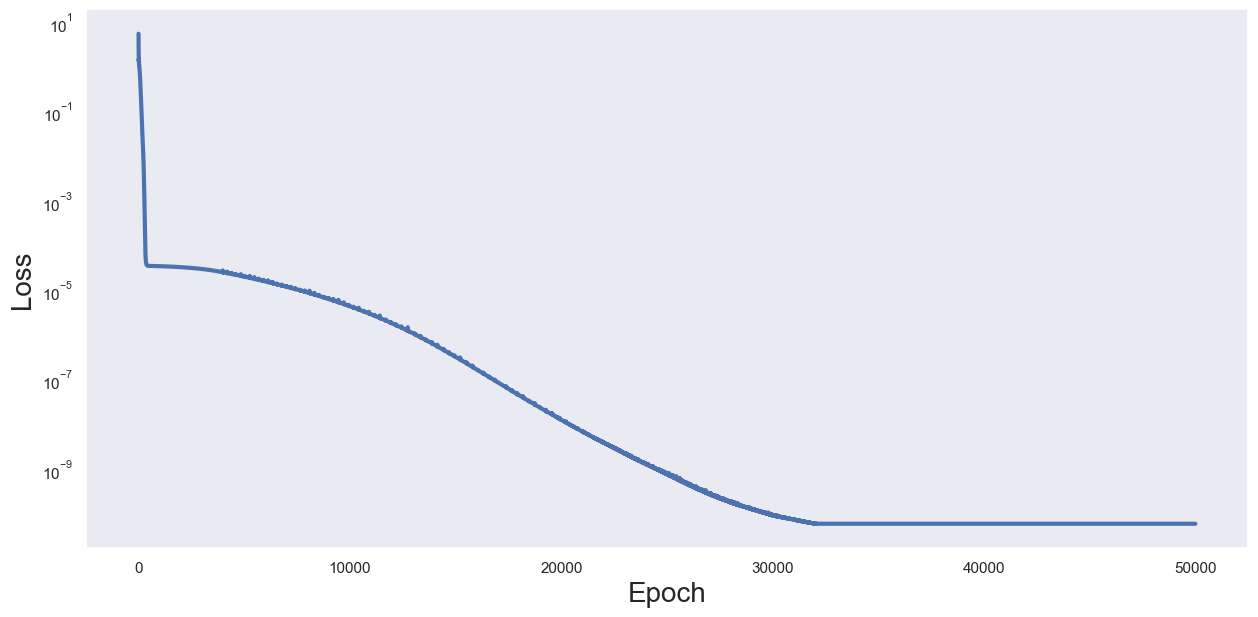
\includegraphics[width=\linewidth]{img//chapter5//sersic/loss_sersic.png}
    \caption[Loss function vs epochs for Sérsic profile fit]{Loss function vs epochs for the training of the Sérsic model.}
    \label{fig:loss_sersic}
\end{figure}

After training the model, an estimation of parameter errors was performed throughout MCMC sampling, using the Pyroframework. Pyro is a probabilistic programming language built on top of PyTorch, designed to create and run complex probabilistic models. It offers tools for defining flexible and expressive Bayesian models and algorithms for variational inference, making it well-suited for tasks in machine learning and statistics that involve uncertainty. Pyro's integration with PyTorch allows for automatic differentiation and GPU acceleration, enabling efficient and scalable model fitting and evaluation.

The probabilistic model was defined with a uniform distribution for the parameters, and then $5000$ samples from the posterior distributions were extracted. Their mean values and standard deviations are described in \cref{tab:parameters_2}.

\begin{table}[]
\setlength{\extrarowheight}{2pt}
\setlength{\tabcolsep}{1pt}
\centering
\caption{Summary of true, initial and best-fit parameters.}
\label{tab:parameters_2}
%\resizebox{0.2\linewidth}{!}{
\begin{tabular}{@{}c@{\hskip 20pt}c@{}@{\hskip 20pt}c@{}@{\hskip 20pt}c@{}@{\hskip 20pt}c@{}}
\toprule
Parameter   & True value            & Initial value             & Best-fit value            & Best-fit value (MCMC) \\ \midrule
$I_e$       & \SI{15.0}{}           & \SI{25.0}{}               & \SI{15.0077}{}            & \SI[separate-uncertainty=true]{14.9777 \pm 0.1499}{} \\
$R_e$       & \SI{2.0}{\arcsecond}  & \SI{4.5}{\arcsecond}      & \SI{1.9997}{\arcsecond}   & \SI[separate-uncertainty=true]{2.0014 \pm 0.0106}{\arcsecond} \\
$n$         & \SI{3.5}{}            & \SI{7.0}{}                & \SI{3.5002}{}             & \SI[separate-uncertainty=true]{3.5080 \pm 0.0376}{} \\
$x_0$       & \SI{0.2}{\arcsecond}  & \SI{12.2}{\arcsecond}     & \SI{0.2000}{\arcsecond}   & \SI[separate-uncertainty=true]{0.2000 \pm 0.0009}{\arcsecond}\\
$y_0$       & \SI{-0.3}{\arcsecond} & \SI{-18.0}{\arcsecond}    & \SI{-0.3000}{\arcsecond}  & \SI[separate-uncertainty=true]{-0.2999 \pm 0.0010}{\arcsecond}   \\
$q$         & \SI{0.6}{}            & \SI{0.8}{}                & \SI{0.5999}{}            & \SI[separate-uncertainty=true]{0.5999 \pm 0.0014}{}  \\
$\varphi$   & \SI{0.7853}{\radian}  & \SI{1.5708}{\radian}      & \SI{0.7854}{\radian}      & \SI[separate-uncertainty=true]{0.7854 \pm 0.0018}{\radian}\\ \bottomrule
\end{tabular}
%}
\end{table}

\Cref{fig:corner_sersic} shows the corner plot to illustrate the multidimensional distributions of and between the parameters. Diagonal elements consist of histograms representing the marginal distributions of individual parameters. They allow one to discern the central tendencies (such as mean or median), the spread (variance or standard deviation), and the shape (indications of skewness or multiple peaks) of each parameter's distribution. Off-diagonal elements display the joint distributions between pairs of parameters through contour plots. They are instrumental in understanding the correlations or dependencies between parameters, with circular patterns indicating minimal correlation and elongated ellipsoids suggesting strong correlations. The orientation of these ellipsoids further clarifies the nature of the relationship, be it positive or negative.

In particular, the corner plot shows the correlation between some parameters involved. As is known from the literature \citep{graham_concise_2005,ciotti_analytical_1999}, the Sérsic profile presents degeneracies between some of its parameters:
\begin{itemize}
    \item intensity $I_e$ and effective radius $R_e$: larger radius with lower intensity can produce a similar overall brightness as a smaller radius with higher intensity;
    \item Sérsic index $n$ and effective radius $R_e$: galaxies with higher Sérsic indices tend to also have larger effective radii, as both parameters are related to how light is distributed in a galaxy.
\end{itemize}
Additionally, \cite{trujillo_effects_2001,trujillo_effects_2001-1} showed that in addition to the intrinsic degeneracies among the Sérsic parameters, there are some further degeneracies between the latter and the PSF. One can think of the intrinsic galaxy axis ratio as a very intuitive example. The PSF is, by definition, rounder than a flattened galaxy; hence, its effect on the two-dimensional light distribution produces a rounder galaxy. The higher the FWHM in arcsecs, the rounder the observed galaxy is \citep{peng_detailed_2002,li_galaxy_2022}.

\begin{figure}
    \centering
    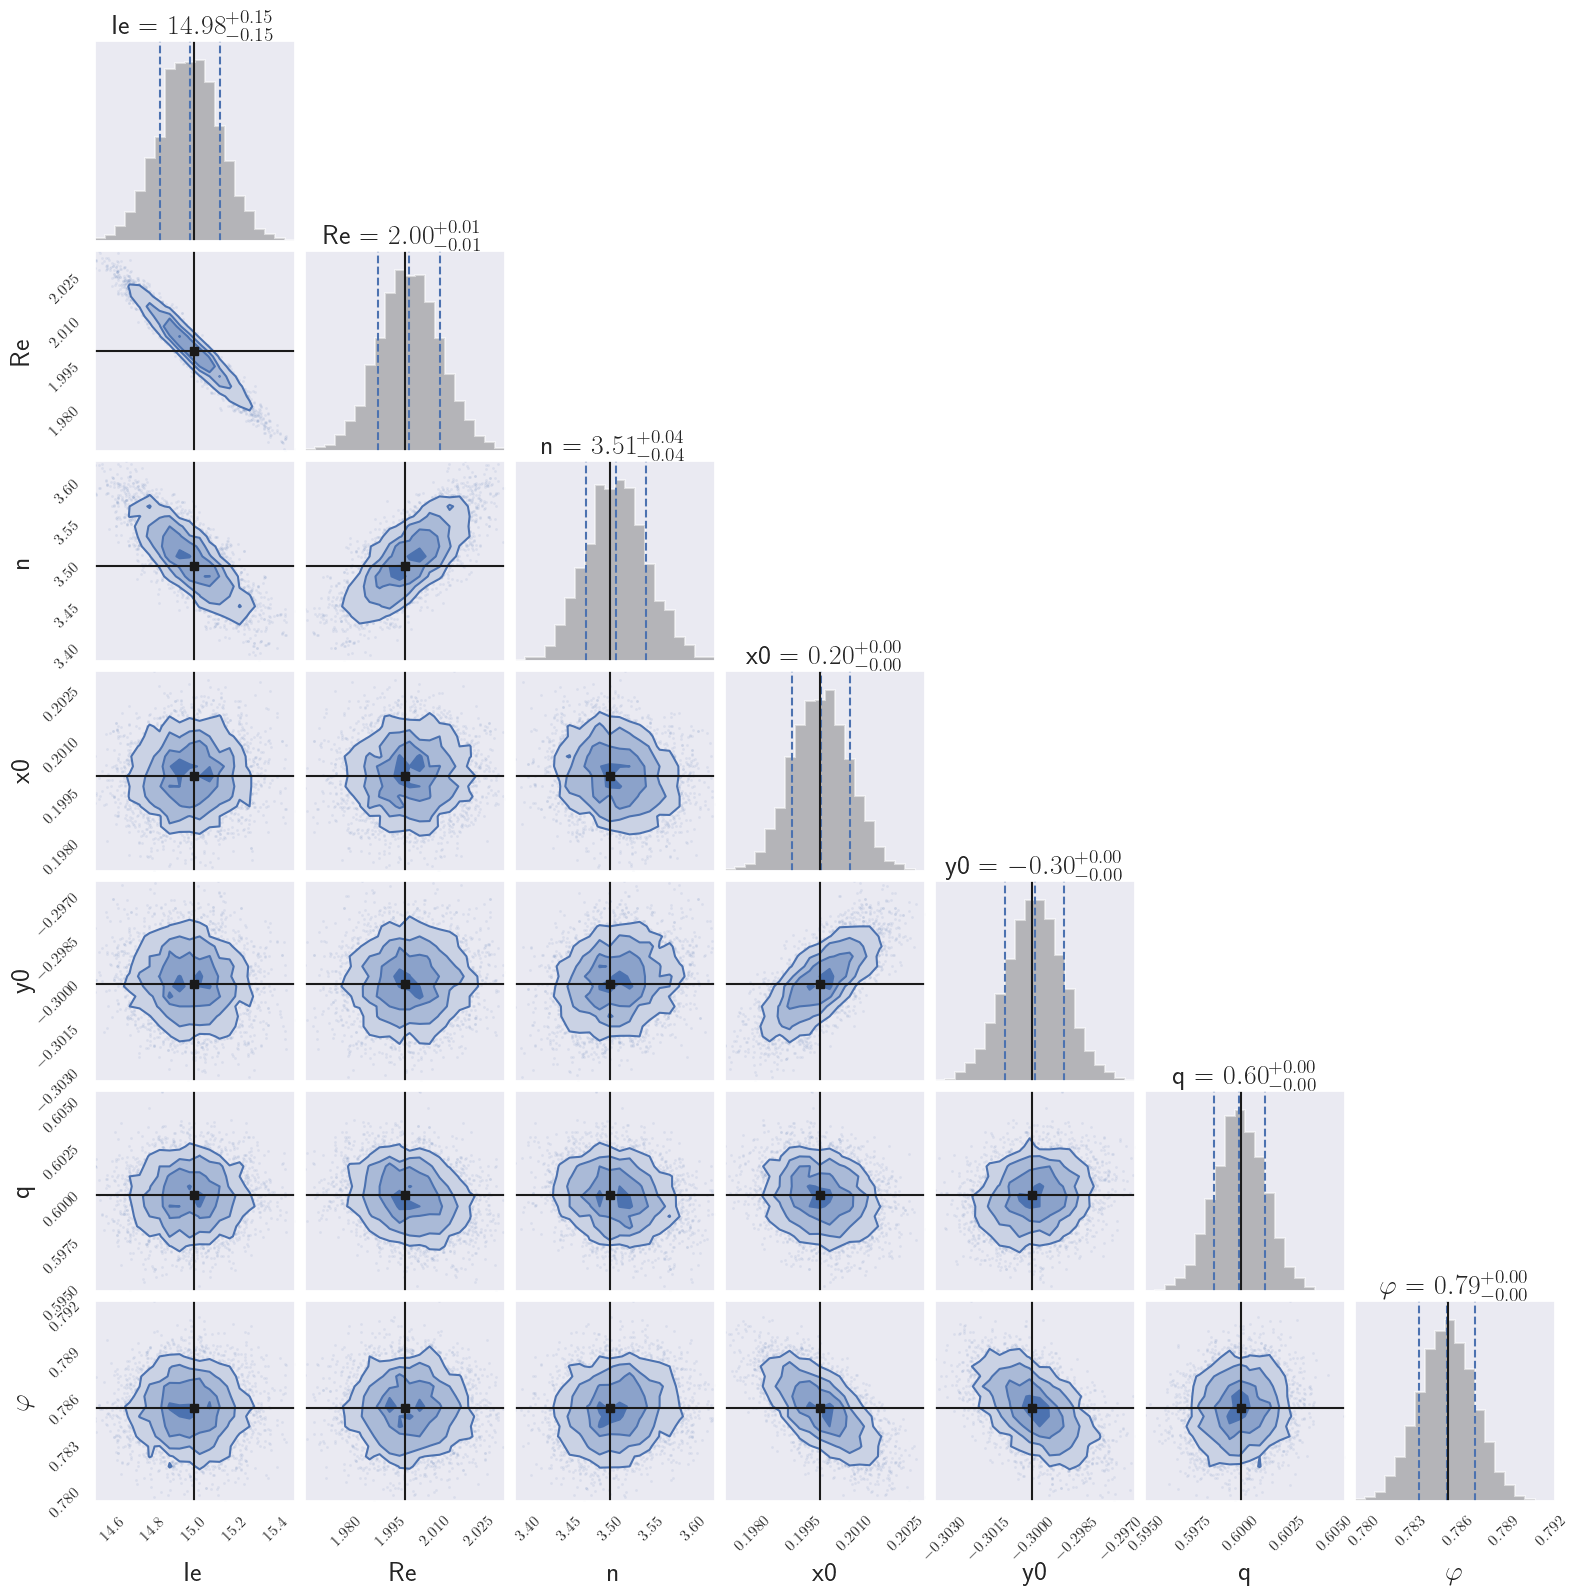
\includegraphics[width=\linewidth]{img//chapter5//sersic/corner_sersic.png}
    \caption[Corner plot Sérsic profile]{Corner plot showing the posterior probability distributions of the parameters used to fit the Sérsic surface brightness profile. The projections of the probability density on planes defined by each couple of parameters are shown, as well as one-dimensional marginalized distributions. The black and the blue dashed vertical lines in one-dimensional histograms indicate the true values and the 16th, 50th and 84th percentiles of the distributions.}
    \label{fig:corner_sersic}
\end{figure}